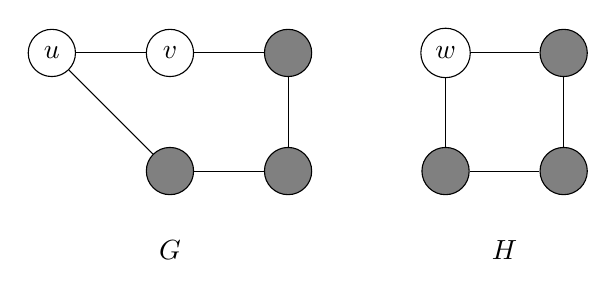
\begin{tikzpicture}

\node[circle, minimum height=0.6cm, draw] (v1) at (0,0) {$u$};
\node[circle, minimum height=0.6cm, draw] (v2) at (1.5,0) {$v$};
\node[circle, minimum height=0.6cm, draw, fill=gray] (v3) at (3,0) {};
\node[circle, minimum height=0.6cm, draw, fill=gray] (v5) at (1.5,-1.5) {};
\node[circle, minimum height=0.6cm, draw, fill=gray] (v4) at (3,-1.5) {};
\draw  (v1) edge (v2);
\draw  (v2) edge (v3);
\draw  (v3) edge (v4);
\draw  (v4) edge (v5);
\draw  (v5) edge (v1);

\node[circle, minimum height=0.6cm, draw] (v6) at (5,0) {$w$};
\node[circle, minimum height=0.6cm, draw, fill=gray] (v7) at (6.5,0) {};
\node[circle, minimum height=0.6cm, draw, fill=gray] (v8) at (6.5,-1.5) {};
\node[circle, minimum height=0.6cm, draw, fill=gray] (v9) at (5,-1.5) {};
\draw  (v6) edge (v7);
\draw  (v7) edge (v8);
\draw  (v8) edge (v9);
\draw  (v9) edge (v6);

%\node (v10) at (3.5,-0.75) {};
%\node (v11) at (4.5,-0.75) {};
%\draw[->, line width=0.05cm]  (v10) edge (v11);
\node at (1.5,-2.5) {$G$};
\node at (5.75,-2.5) {$H$};
\end{tikzpicture}